\documentclass[frontgrid]{flacards}
\usepackage{color}
\usepackage{tabularx}
\usepackage{graphicx}
\usepackage{amsmath}
\definecolor{light-gray}{gray}{0.75}

\newcommand{\frontcard}[1]{\textcolor{light-gray}{\colorbox{light-gray}{$#1$}}}
\newcommand{\backcard}[1]{#1} 

\newcommand{\flashcard}[1]{% create new command for cards with blanks
    \card{% call the original \card command with twice the same argument (#1)
        \let\blank\frontcard% but let \blank behave like \frontcard the first time
        #1
    }{%
        \let\blank\backcard% and like \backcard the second time
        #1
    }%
}

\begin{document}

\pagesetup{2}{4} 

%\card{
%	The MU0 is a 16 bit architecture, what two parts are in each instruction, and
% how large are they?
%}{
%	4 bits for an operation and 12 for the address.
%}
%
%\card{
%	In the MU0, what are the two programmer visible registers?
%}{
%	The program counter and the accumulator.
%}
%
%\card{
%	How many bits long is the program counter and what does it store?
%}{
%	12 bits, stores the address in memory of the next instruction to be executed.
%}
%
%\card{
%	How many bits is the accumulator and what does it store?
%}{
%	16 bits, stores the result of the last arithmetic operation.
%}
%
%\card{
%	What happens when `LDA s' is run?
%}{
%	ACC = [s]
%}
%
%\card{
%	What happens when `STA s' is run?
%}{
%	[s] = ACC
%}
%
%\card{
%	What happens when `ADD s' is run?
%}{
%	ACC += [s]
%}
%
%\card{
%	What happens when `SUB s' is run?
%}{
%	ACC -= [s]
%}
%
%\card{
%	What happens when `JMP s' is run?
%}{
%	PC = s
%}
%
%\card{
%	What happens when `JGE s' is run?
%}{
%	if ACC >= 0 then PC = s
%}
%
%\card{
%	What happens when `JNE s' is run?
%}{
%	if ACC != 0 then PC = s
%}
%
%\card{
%	Briefly explain what the fetch-execute cycle is.
%}{
%	The next instruction is fetched from memory (at the address pointed to by the PC), then the instruction is executed.
%}
%
%\card{
%	What three steps occur during the fetch phase?
%}{
%	\begin{tabularx}{0.32\textwidth}{l X}
%		1. & Read the data stored in the address that the PC is pointing to.\\
%		2. & Save result of read in the instruction register\\
%		3. & Increment the PC.
%	\end{tabularx}
%}
%
%\card{
%	In order for every instruction to run smoothly what needs to be worked out?
%}{
%	\begin{tabularx}{0.32\textwidth}{l X}
%		1. & The critical path for each operation.\\
%		2. & The time allowed for signals to propagate through even the longest critical path.\\
%	\end{tabularx}
%}

%\card{
%	What control signals do all registers need?
%}{
%	An enable signal
%}
%
%\card{
%	What control signal does a multiplexer need?
%}{
%	A signal to select an input
%}
%
%\card{
%	What control signals does the memory need?
%}{
%	Ren (read enable) and Wen (write enable)
%}
%
%\card{
%	Which 3 signals control the ALU?
%}{
%	add, sub \& byp
%}

\card{
	What two jobs do operating systems do in general?
}{
	\begin{tabularx}{0.32\textwidth}{l X}
		1. & Manage the resources of the system.\\
		2. & Abstract the implementation of the system from the running programs.\\
	\end{tabularx}
}

\card{
	What is a process?
}{
	A program in execution, the thread + address space.
}

\card{
	What is the address space?
}{
	All memory locations the process can use.
}

\card{
	What is a thread?
}{
	A sequence of instructions that are obeyed.
}

\card{
	What is multi-threading?
}{
	This is where we have multiple threads within the same process
}

\card{
	How do we make programs think they have sole use of memory?
}{
  Use \textbf{relocation}, where we provide a virtual machine for each program,
  allowing them to behave as though they have sole use of memory. We need to
  support some kind of virtual memory for this.
}

\card{
	What are the two most common modes of operation?
}{
	User and system
}

\card{
	What are the three different approaches to engineering an OS?
}{
	Monolithic, layered and micro-kernels.
}

\card{
	What are the three process states?
}{
	Running, ready, blocked
}

\card{
	In the diagram, what is happening at each stage?\\
	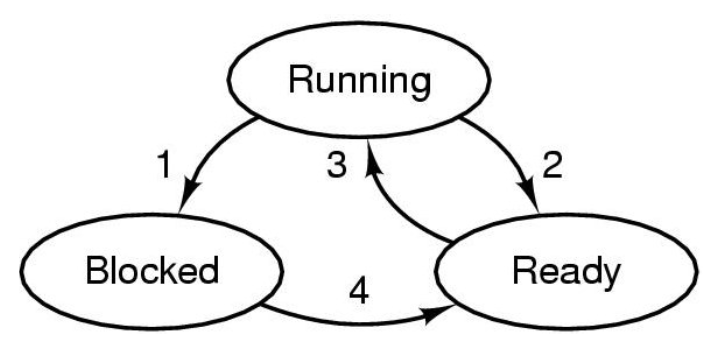
\includegraphics[scale=0.5]{images/processLife.png}
}{
	\begin{tabularx}{0.32\textwidth}{l X}
		1. & Process needs to wait for I/O or event.\\
		2. & Process forcibly preempted - \textbf{interrupt / relinquish CPU / time-slice expired}.\\
		3. & Scheduler selects process to run.\\
		4. & I/O or event occurs.\\
	\end{tabularx}
}

\card{
	What is a PCB table?
}{
	Process control block, it contains all of the information needed about processes.
}

\card{
	In scheduling, what do the following mean?
	\begin{tabularx}{0.32\textwidth}{l X}
		1. & CPU burst\\
		2. & I/O burst\\
		3. & CPU bound\\
		4. & I/O bound\\
	\end{tabularx}
}{
	\begin{tabularx}{0.32\textwidth}{l X}
		1. & Process executing on CPU\\
		2. & Process blocked, waiting for I/O\\
		3. & Long CPU bursts\\
		4. & Short CPU bursts\\
	\end{tabularx}
}

\card{
	What is a processes turnaround time?
}{
	The time from a process being submitted to it getting completed.
}

\card{
	What is a processes waiting time?
}{
	The time that the process waits to run.
}

\card{
	Briefly explain the first come first served scheduling algorithm.
}{
	The first process in the ready state gets CPU time first. Once it is blocked or complete, the next process in the queue is run. Processes that require CPU time are added to the back of the queue.
}

\card{
	Briefly explain the shortest remaining time first scheduling algorithm.
}{
	For each newly ready process, if CPU-burst is less than the time to complete the running process then context-switch and run the new process.
}

\card{
	What is meant by non-pre-emptive scheduling?	
}{
	Scheduling where processes run until they are terminated or blocked.
}

\card{
	What is meant by pre-emptive scheduling?
}{
  A pre-emptive scheduler will temporarily interrupt a process, without
  requiring its cooperation, so that other processes can execute, and with the
  intention of resuming the task at a later time. The interrupted process is set
  in the `ready' state so that it can be started again later.
}

\card{
	What is the maximum length a process will be allowed to execute for called in
  pre-emptive processing?
}{
	The `time-slice' or `time-quantum'.
}

\card{
	What is process starvation?
}{
	When the scheduling algorithm leaves a process out for a long time, causing the process to not receive any CPU time.
}

\card{
	In scheduling, what are static priorities?
}{
	Priorities that are predetermined for each process.
}

\card{
	In scheduling, what are dynamic priorities?
}{
	Priorities that are assigned by the system to achieve certain goals.
}

\card{
	What is a race condition?
}{
	When one or more processes/threads execute in parallel, but the outcome depends on which finishes first.
}

\card{
	What do the following terms mean?
	\begin{tabularx}{0.32\textwidth}{l X}
		1. & Data inconsistency\\
		2. & Synchronisation\\
		3. & Critical section\\
		4. & Mutual exclusion\\
	\end{tabularx}
}{
	\begin{tabularx}{0.32\textwidth}{l X}
		1. & Disagreement about data values\\
		2. & Using appropriate policies and mechanisms to ensure the correct operation of cooperating processes\\
		3. & Section of code in which shared data is used\\
		4. & At most 1 process can be in its critical section at once\\
	\end{tabularx}
}

\card{
	What is deadlock?
}{
	Where there are a set of waiting processes where each process is waiting for something that can only be provided by another of the processes.
}

\card{
	What is the base register of a program?
}{
	A register that is loaded with the physical address where the program begins in memory.
}

\card{
	What is the limit register of a program?
}{
	A register that is loaded with the length of the program.
}

\card{
	What is the base register usage sequence?
}{
	When the processor references memory, either fetch an instruction or read or write a data word, the CPU hardware automatically adds the base value to the address generated by the processor before sending the address out on the memory bus.
}

\card{
	What is the limit register usage sequence?
}{
	When the base register usage sequence happens, the OS checks if the address offered is greater than the value in the limits register, in which case a fault is generated and access aborted.
}

\card{
	What is the virtual address?
}{
	An address that is generated by a program. It is converted to the actual `physical address' which is used in memory.
}

\card{
	What performs the virtual to physical address conversion?
}{
	The memory management unit (MMU)
}

\card{
	What are the two main reasons for virtual memory in a computer system?
}{
	\begin{tabularx}{0.32\textwidth}{l X}
		1. & To allow a processor to address a much larger address space than is implemented by the physical memory\\
		2. & To support the OS in the management of processes\\
	\end{tabularx}
}

\card{
	What is a page table?
}{
	A table used by the MMU to translate from a virtual to a physical address.
}

\card{
	What are the two techniques used to implement virtual memory?
}{
	Paged virtual memory and segmented virtual memory.
}

\flashcard{
	Segmented memory is split into chunks of a \blank{variable} size.
}

\card{
	What is the formula to work out the number of pages used in a system?
}{
	\[\#pages = \frac{addressSpace}{PageSize}\]
	Where $addressSpace$ and $pageSize$ are measured in bits.
}

\card{
	What is the format of an address to paged memory?
}{
	Page number + offset
}

\card{
	What steps does the MMU take when it receives a paged address?
}{
	\begin{tabularx}{0.32\textwidth}{l X}
		1. & Look up the page number in the page table and see if it's in physical memory.\\
		2. & If it is in memory, generate a physical address $\text{page-base address} + \text{offset}$, and request that from RAM.\\
		3. & If it's not, abort the memory access, OS will load the page into memory (this is a page fault).
	\end{tabularx}
}

\card{
	What columns are present in the page table?
}{
	\begin{tabularx}{0.32\textwidth}{l X}
		- & Resident flag\\
		- & Used flag\\
		- & Dirty flag\\
		- & Physical address\\
		- & Disk address\\
	\end{tabularx}
}

\flashcard{
	In a page table, the resident flag checks whether the page is \blank{currently
  in memory}
}

\flashcard{
	In a page table the used flag check whether the page \blank{has been used}
}

\card{
	In a page table, what does the dirty flag do?
}{
	Checks whether the page has been written to while it's been in physical memory (so it needs to be copied back in full when it's put back onto the disk).
}

\card{
	LRU is a page replacement algorithm, what does LRU stand for?
}{
	Last recently used
}

\card{
	FIFO is a page replacement algorithm, what does FIFO stand for?
}{
	First in first out.
}

\card{
	Briefly explain what the FIFO page replacement algorithm does.
}{
	Identifies the oldest page in memory and gets rid of it.
}

\card{
	Briefly explain what the second chance page replacement algorithm does.
}{
	This picks the oldest page with the fewest number of accesses since the last
  pass of the algorithm.
}

\card{
	Briefly explain the last recently used page replacement algorithm.
}{
	This picks the page that has been used the longest ago. It's implemented using 
  a timestamp that is updated when the page is read or written to.
}

\card{
	What is a write-back?
}{
	When we write a page back to the disk when we swap it out.
}

\card{
	What are two attributes that segments have that define how they are used?
}{
	Usage rights and access rights.
}

\card{
	When does a segment fault occur?
}{
	When the OS tries to access a segment that is not in memory.
}

\card{
	Explain external fragmentation.
}{
	When segments are moved in and out of main memory, `holes' appear in the
  memory (due to segments having different sizes), which reduces the amount of
  useful memory.
}

\card{
	What can we do to prevent fragmentation?
}{
	Use algorithms to find a good place to put segments, such as `best fit' and
  `first fit' when the OS is placing segments in memory.
}
\end{document} 
